\section{Where Do Memory Scores Come From?}
\label{sec:audit}
% A/B: 4.1-4.2 passed in round 2, 4.3-4.4 in round 3. 10-17 user request: fewer inline numbers, figures instead of
% tables; intervals moved to the appendix (\cref{app:detail}).

Before proposing a method, we use the protocol of \cref{sec:setting} to measure how much of a memory system's score
comes from the memory and how much from its surroundings. All numbers in this section are on development sets with
gpt-6-luna as reader and judge; intervals for every difference are in \cref{app:detail}. With 100 BEAM-1M or 200
BEAM-100K questions, single-run differences below about 4 points are not resolved.

% A1: prompt
\subsection{The answer prompt shifts scores by several points}
\label{sec:audit-prompt}
\Cref{tab:prompt} keeps every context fixed and changes only the answer prompt. The prompt that Mem0 released for
BEAM raises Hindsight on BEAM-1M by about 9 points in one run (about 5 over three runs) and record retrieval by about
4; on BEAM-100K it helps both memories by about 2 points and lowers the full-context reader by 4. None of the resulting
rank changes is resolved, so we claim only that the answer prompt moves absolute scores by as much as many published
differences between systems, not that it reorders the systems we test. We use the tuned prompt in the rest of the
paper because it is the public answer prompt for BEAM, and neither prompt was adjusted on our development questions.

\begin{table}[t]
\centering\small
\caption{Changing only the answer prompt (one run each, contexts unchanged). Minimal: our plain prompt; tuned: the BEAM
answer prompt released by Mem0; CC: conflict check. Intervals in \cref{app:detail}.}
\label{tab:prompt}
\begin{tabular}{lrrrrrr}
\toprule
& \multicolumn{3}{c}{BEAM-100K} & \multicolumn{3}{c}{BEAM-1M} \\
\cmidrule(lr){2-4}\cmidrule(lr){5-7}
System & minimal & tuned & $\Delta$ & minimal & tuned & $\Delta$ \\
\midrule
Full context & \prelim{69.9} & \prelim{65.9} & \prelim{$-4.0$} & --- & --- & --- \\
Record retrieval\,+\,CC & \prelim{67.5} & \prelim{69.7} & \prelim{$+2.2$} & \prelim{64.6} & \prelim{68.7} & \prelim{$+4.1$} \\
Hindsight & \prelim{66.5} & \prelim{69.1} & \prelim{$+2.6$} & \prelim{63.7} & \prelim{72.3} & \prelim{$+8.6$} \\
\bottomrule
\end{tabular}
\end{table}

\begin{figure}[t]
\centering
\begin{subfigure}[b]{0.47\linewidth}\centering
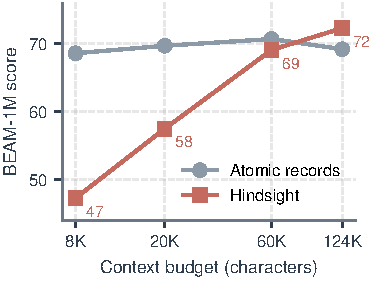
\includegraphics[width=\linewidth]{figs/fig3_budget.pdf}
\caption{Score against context budget.}\label{fig:budget}
\end{subfigure}\hfill
\begin{subfigure}[b]{0.50\linewidth}\centering
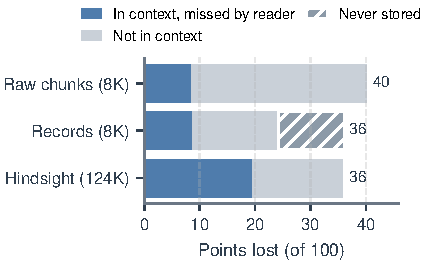
\includegraphics[width=\linewidth]{figs/fig4_loss.pdf}
\caption{Where the lost points go.}\label{fig:loss}
\end{subfigure}
\caption{\textbf{Budget and reader, not storage format, separate the systems on BEAM-1M} (100 development questions,
one run). (a) Atomic records score about the same at every budget; Hindsight needs its full 124K characters. (b) The
8K systems lose most points to information that never reached the reader; Hindsight loses about half of its points to
information that was in its context.}
\label{fig:audit}
\end{figure}

% A2: budget x format
\subsection{Hindsight needs a large context budget; atomic records do not}
\label{sec:audit-budget}
Hindsight stores narrative facts with entity summaries and hands the reader 124K characters; record retrieval stores
atomic records and hands it 8K. \Cref{fig:budget} separates format from budget by cutting each system's ranked
context, at memory boundaries, to the same length. Atomic records stay within about 2 points of each other from 8K to
124K characters. Hindsight falls to 47 at 8K, about 21 points below records, is level with them from 60K on, and is
ahead by 3 points at 124K in this run. The steep curve has a likely mechanical cause: Hindsight's top-ranked memories
carry long raw excerpts, and an 8K cut keeps a median of 2 of its 223 retrieved memories. A comparison of the two
systems at their default settings therefore confounds the format with the budget.

% A3: where the points are lost
\subsection{The 8K systems lose points at retrieval, Hindsight about half at the reader}
\label{sec:audit-loss}
For every rubric item an answer misses, we ask gpt-6-luna whether the information the item needs appears in the
context the reader received and, for record retrieval, whether it appears anywhere in the stored records. A second
judge, gpt-6.1-sol, agrees on 92\% of a 50-item sample for each 8K system and on 76\% for Hindsight, whose long
contexts are harder to check; where they disagree on Hindsight, gpt-6.1-sol more often finds the information in
context, so the reader share below is, if anything, an underestimate. \Cref{fig:loss} shows the split on BEAM-1M. The
two 8K systems lose most of their points before the reader sees anything: raw-chunk retrieval loses 32 of its 40
points to information missing from its context, and record retrieval loses 15 to records that were stored but not
retrieved and 12 to information no record holds. Hindsight's longer context does not lower the total loss (36 points),
but about half of it (20 points) comes from information that was in front of the reader. Because the three systems
differ in more than context length, this describes where they lose points rather than testing whether length causes
reader errors. Raw text is not the remedy either: at a 20K-character budget, replacing each retrieved record with the
dialogue turns it came from lowered BEAM-100K by about 10 points (one run, 120 questions).

% A4: write-time changes
\subsection{The write-time changes we tried did not raise scores}
\label{sec:audit-write}
Before turning to the read side, we tried three changes to what the record store keeps, each on BEAM-100K with record
retrieval as the base. Anchoring each record to verbatim quotes did not change the score over three runs. Keeping both
sides of every contradiction instead of resolving one lowered contradiction questions, because the reader still
ignored the conflict: both statements reached it in 14 of 20 questions, and it raised the conflict in only about half
of those. Keying records by proposition, so that later statements would chain to earlier ones, failed before any
answer was produced, because the two sides of a contradiction never received the same key. Rewriting the store in
place was worse than leaving it alone. In a drift test on LoCoMo, a summary rewritten after every session ended about
20 points below a summary of the same length rebuilt from the untouched ledger, and on BEAM-1M even gpt-6.1-sol, writing
an 8K summary, kept fewer ledger facts when it rewrote than when it rebuilt. \Cref{app:detail} gives counts and tests.
These results do not rule out better write-time designs, but they point to the read side, where \cref{fig:loss} places
about half of the losses of the one system with a long context.
